\section{Deployment}
\subsection{Allgemein}
\subsection{Cloudfoundry}
\subsection{Docker}\label{Docker}
Die in Absatz \ref{rabbitmq} erläuterte message-oriented Middleware RabbitMQ wird als Docker Container deployed. Durch die Verwendung von Docker Containern ist es möglich, lauffähige Software in isolierten Containern zu starten. Dies hat den Vorteil, dass die Software immer in identischen Umgebungen gestartet wird, unabhängig davon ob der Container lokal auf dem Entwicklungsrechner oder auf dem Produktivsystem läuft. Dies betrifft auch die Abhängigkeiten von notwendigen Installationen. So basiert RabbitMQ wie in Absatz \ref{rabbitmq} erwähnt auf der Sprache Erlang, weshalb diese auf jedem Entwicklungs- und Produktivsystem installiert werden müsste. Durch die Verwendung von Docker können notwendige Installationen bereits im Dockerfile definiert werden. So wird beispielsweise die Installation von Erlang in Abb. \ref{img:erlangDockerfile} veranschaulicht. 

\begin{figure}[htbp]
	\centering
	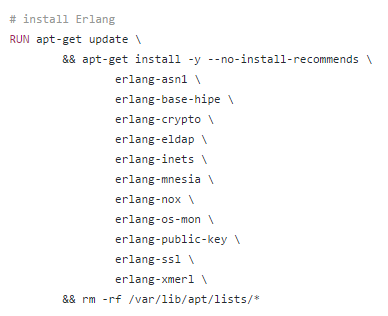
\includegraphics[width=0.5\textwidth]{Bilder/erlangDockerfile.png}
	\caption{Installation von Erlang im Dockerfile Quelle: https://github.com/docker-library/rabbitmq/blob/a6cb36022a5c1a17df78cfafe45a73d941ad4eb8/3.6/\-debian/Dockerfile}
	\label{img:erlangDockerfile}
\end{figure}
Dies ist ein Ausschnitt aus dem Dockerfile des offiziellen Rabbitmq-Baseimages, einer Abbildung des Containers. Der Abschnitt stellt die Installation von Erlang auf einem Linux-System unter Verwendung des Paketmanagers \textit{Advanced Packaging Tool} (APT) dar.
\subsubsection{Dockerfile}
Das Dockerfile für diesen Use-Case besteht neben dem erwähnten Baseimage aus Aktivierungen des in Absatz \ref{rabbitmq} vorgestellten Management Plugins, des MQTT Plugins sowie des MQTT-Websocket Plugins. Durch die Verwendung des Websocket Plugins ist die Kommunikation mit RabbitMQ auch über Webseiten möglich. Ein weiterer Bestandteil des Dockerfiles ist die rabbitmq.config. Diese ist notwendig um den Zugriff auf die MOM einzuschränken, da andernfalls eine Default-Konfiguration verwendet werden würde und durch diese der Nutzer \emph{guest} vollen Zugriff hätte. Um dennoch Administrations-Zugriff zu erlangen, wird über das Shell-Skript \textit{init.sh} ein Nutzer mit Administratorrechten angelegt. Die Zugangsdaten dieses Nutzers sind als Umgebungsvariablen hinterlegt. Die Ausführung des Skripts wird über den CMD-Befehl des Dockerfiles gesteuert. Zusätzlich ist es notwendig, Docker über den Befehl EXPOSE zu informieren, welche Ports der Container abhört. Im Anschluss an die Erstellung des Dockerfiles kann durch den Befehl \emph{docker build} ein Image erzeugt werden. Dieses Image wird auf den Amazon Container Service deployed.
\subsubsection{Amazon Container Service}\label{acs}
Dabei handelt es sich um einen hoch skalierbaren Container Managementservice welcher eine unkomplizierte Handhabung von Docker Containern in Amazon EC2 Instanzen anbietet. Die Erstellung eines Clusters ist in wenigen Schritten möglich. Zunächst wird ein Repository zur Speicherung des erstellten Images angelegt. Im Anschluss daran kann nach der erforderlichen Installation des Amazon Web Service Command Line Interfaces (AWS CLI) der Zugriff auf das Repository erfolgen. Nachdem das Image gepusht wurde, muss die Task Definition erstellt werden. Dabei handelt es sich um eine Anleitung für den Start des Containers. Ein Bestandteil der Task Definition ist das Port Mapping. Dabei wird dem Service mitgeteilt, wie die im Dockerfile deklarierten Ports ausserhalb des Containers erreichbar sein sollen. Zusätzlich werden in den erweiterten Optionen die Umgebungsvariablen und somit die Zugangsdaten für den in der \emph{init.sh} erstellten Administator hinterlegt. Im nächsten Schritt erfolgt die Konfiguration des Services, in welcher ein Load Balancer erstellt und ausgewählt werden kann. Im abschließenden Schritt erfolgt die Konfiguration des eigentlichen Clusters. Hierbei erfolgt die Auswahl der Art und der Anzahl des gewünschten Instanz Typs. Durch diesen wird festgelegt, welche Resourcen für eine einzelne Instanz verfügbar sein werden. Darüber hinaus kann in diesem Abschnitt ein Schlüsselpaar für den SSH-Zugriff erstellt und ausgewählt werden. Erfolgt dies nicht, ist kein Zugriff über die EC2 Konsole auf den Container möglich. Die Skalierbarkeit erfolgt durch den optionalen Auto Scaling Service. Dieser kann dahingehend konfiguriert werden, dass die minimale, eine maximale und eine gewünschte Anzahl Instanzen pro Task festgelegt wird.

\subsection{Heroku}\label{Heroku}
Der Webclient wird als PHP-Anwendung bei Heroku deployed. Wird eine Änderung im konfigurierten Git-Repository  im angegebenen Branch erkannt wird ein neuer Build ausgelöst und die Applikation neu deployed. Als Serverregion ist Europa angegeben, dies führt zu einem deployment in Irland wodurch gute Antwortzeiten im europäischen und auch noch akzeptable Antwortzeiten an der US-amerikanischen Ostküste erreicht werden können. Die für die Entwicklung genutzte kostenlose Instanz fährt nach 30 Minuten ohne Anfrage automatisch herunter, für den Produktiveinsatz wäre somit zu Beginn der Plan "Hobby" sinnvoll, der bei Inaktivität nicht abschaltet. Werden mehr als 1500 Aufrufe pro Sekunde erwartet muss auf den "Professional" Plan umgestellt werden, welcher dann das horizontale Skalieren über mehrere Serverinstanzen erlaubt. Die Skalierung kann über das Heroku Command Line Interface (CLI) gesteuert werden bzw. ab einem "Performance M" Server auch lastabhängig voll automatisch von Heroku gesteuert werden. Die Umgebungsvariablen für die Zugangsvariablen zur MOM zu setzten erlaubt Heroku über das Webinterface, wie in Abb. \ref{img:herokuConf} zu sehen, sowie das CLI.
\begin{figure}[htbp]
	\centering
	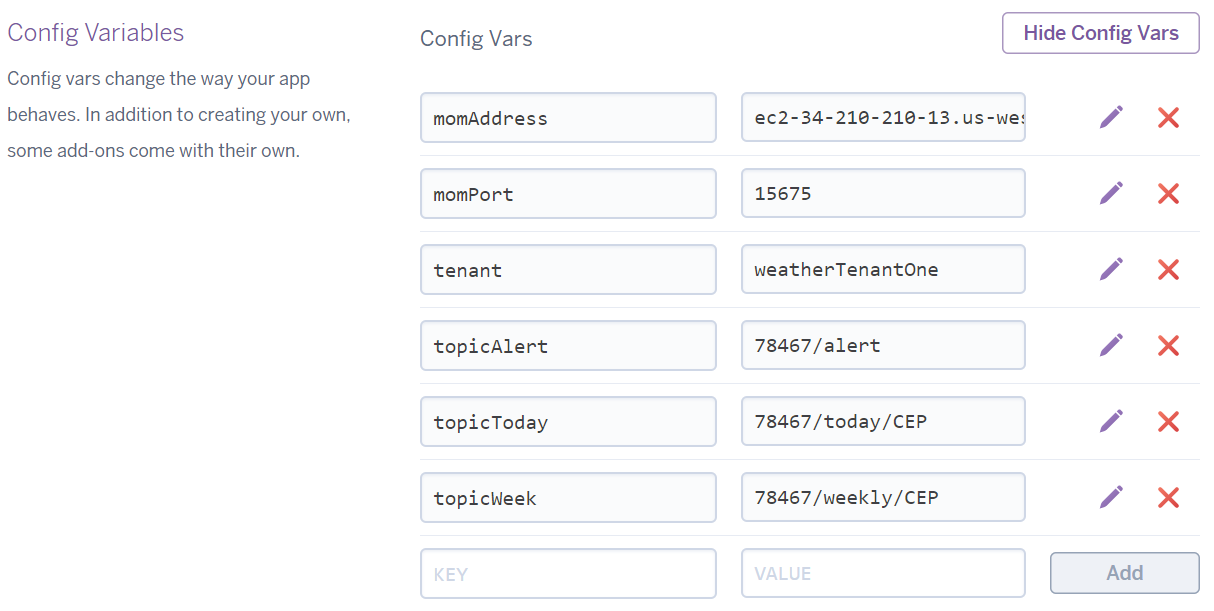
\includegraphics[width=1.0\textwidth]{Bilder/Web-herokuEnv.PNG}
	\caption{Konfiguration der Variablen bei Heroku}
	\label{img:herokuConf}
\end{figure} 


\subsection{REDIS}
\subsection{AWS}